\section{Aufgabe 8}
\begin{equation}
  f(x)=\frac{x^3}{e^x-1}
\end{equation}
\subsection{Teilaufgabe a)} \label{sec:8a}
\begin{figure}[H]
  \centering
  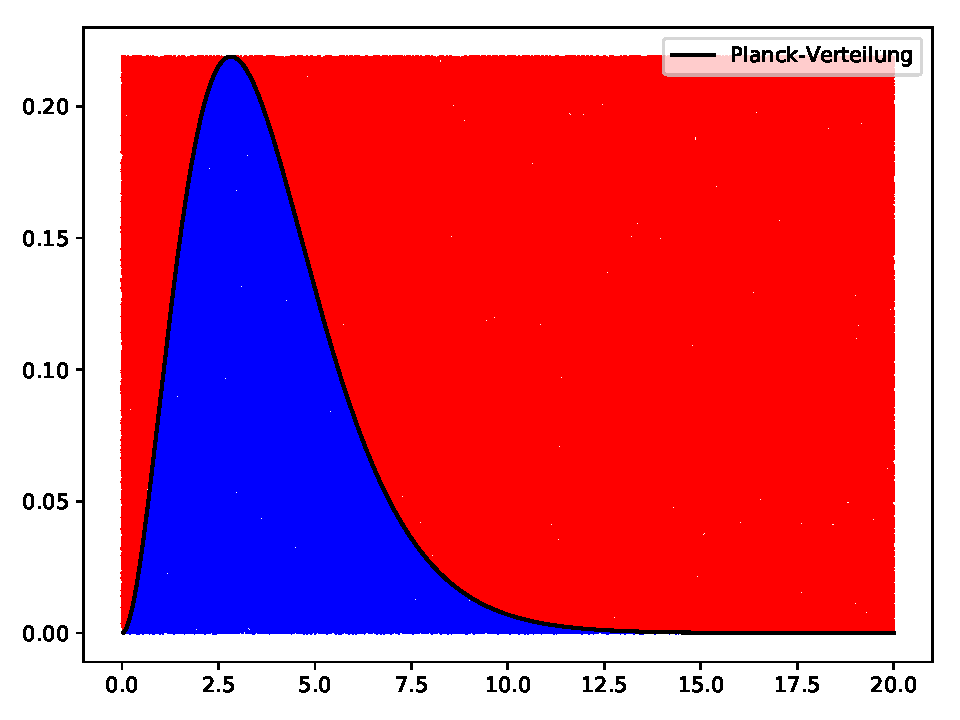
\includegraphics{Aufgabe08/a.pdf}
  \caption{Rückweisungsmethode a)}
  \label{fig:rwm1}
\end{figure}
Rückweisungsverfahren mit der Majorante
\begin{equation}
  g(x)=f(x_{max}) \text{ für } 0 < x < 20 \text{.}
\end{equation}
Dabei ist $x_{max}$ das $x$, bei dem die Funktion $f(x)$ maximal wird.
\subsection{Teilaufgabe b)} \label{sec:8b}
\begin{figure}[H]
  \centering
  \includegraphics{Aufgabe08/b.pdf}
  \caption{Rückweisungsmethode b)}
  \label{fig:rwm2}
\end{figure}

Rückweisungsmethode mit der Majorante
\begin{equation}
  g(x)=
  \begin{cases}
    f(x_{max}) \text{ für }  x < x_s \\
    200N \cdot x^{-0.1} \cdot e^{-x^{0.9}} \: \text{sonst}\\
\end{cases}
\end{equation}

\subsection{Teilaufgabe c)} \label{sec:8c}
\begin{console1}{Vergleich der Teilaufgaben \ref{sec:8a} und \ref{sec:8b}}
  Anzahl der verworfenen Ereignisse: \\
  a) 337158 \\
  b) 56762 \\
  \\
  Laufzeit: \\
  a) 14.09 s \\
  b) 2.40 s \\
  \\
  Verhaeltnisse a)/b): \\
  verworfene Ereignisse: 5.94 \\
  Laufzeit: 5.88 \\
\end{console1}
Wie zu sehen ist, liefert die Majorante aus aus Teilaufgabe \ref{sec:8a} eine ca fast 6 mal längere laufzeit als die Majorante aus Teilaufgabe \ref{sec:8b}.
Darüber hinaus werden in Teilaufgabe \ref{sec:8a} ca. 6 mal mehr Ergebnisse verworfen als in Teilaufgabe \ref{sec:8b}.
Dies war zu erwarten, da die Majorante aus Teilaufgabe \ref{sec:8b} die Funktion besser eingrenzt.
Lediglich die Berechnung von $x_s$ nimmt etwas Zeit in Anspruch, diese ging jedoch nicht in die Zeitmessung ein.
